\documentclass[10pt,a4paper]{book}

\usepackage{ardour,graphicx,afterpage,url,xstring,xcolor,titlepic}

% XXX: format
\newcommand{\button}[1]{#1}
\newcommand{\menu}[1]{\emph{\StrSubstitute{#1}{,}{ $\rightarrow$ }}}
\newcommand{\key}[1]{\emph{\StrSubstitute{#1}{,}{ + }}}
\newcommand{\directory}[1]{\texttt{#1}}
\newcommand{\todo}[1]{\marginpar{\small\texttt{#1}}}

\newcommand{\screenshot}[3]{%
\begin{figure}[ht]%
\begin{center}
\includegraphics[scale=0.5]{screenshots/#1}
\end{center}
\caption{#2}
\label{#3}
\end{figure}}

% Voodoo from http://answers.google.com/answers/threadview?id=282787
\definecolor{ListingGrey}{rgb}{0.8,0.8,0.8}
\makeatletter\newenvironment{listing}{%
   \medskip\begin{lrbox}{\@tempboxa}\begin{minipage}{\columnwidth}\ttfamily}{\normalfont\end{minipage}\end{lrbox}%
   \colorbox{ListingGrey}{\usebox{\@tempboxa}}\medskip%
}\makeatother

\title{Ardour 3 --- A users' manual}
\titlepic{\includegraphics{graphics/ardour_bw.pdf}}
\author{The Ardour Community}
\date{}
\begin{document}

\maketitle


\clearpage
\thispagestyle{empty}

\bigskip
\bigskip
\bigskip

\begin{quote}
\emph{``One of the secrets of life is that all that is really worth the doing is what we do for others''} --- Lewis Carroll (perhaps)
\end{quote}

\bigskip
\bigskip
\bigskip

\begin{quote}
\emph{``If you want to build a ship, don't drum up the men to gather wood, divide the work and give orders.  Instead, teach them to yearn for the vast and endless sea''} --- Antoine de Sant Exup\'ery (possibly)
\end{quote}

\bigskip

\tableofcontents


\chapter{Introduction}

Hello, and welcome to Ardour!

\section{What is Ardour?}

Ardour is an open-source digital audio workstation (DAW) for Linux and
Mac OS~X.

\section{Typographical conventions}

This manual uses special symbols to denote sections which contain
advanced material.  The reader can skip these sections without any
great loss.

\begin{danger}
Tricky parts of the text are marked with a `bend in the road' marker.
They contain extra information which may be of interest to advanced
users.
\end{danger}

\begin{ddanger}
Especially tricky parts of the text are marked with a double
bend-in-the-road marker.  Such sections will only be of interest to
the completist or serious hacker.
\end{ddanger}

When a menu option is discussed, it will look like this:

\menu{Menu option,Submenu option}




\section{About this manual}

This manual is a constantly-evolving work-in-progress.  In other
words, it is not even close to being complete.  Any suggestions for
improvements, content, or comments on parts that do not make sense are
welcome to \url{cth@carlh.net}.

\begin{danger}
For those familiar with `git', the manual's \LaTeX\ source can be
obtained from the git repository linked from
\url{http://carlh.net/ardour}.  Patches to the manual are most welcome.
\end{danger}


\section{Getting help with Ardour}

There are several places that you can get help with using Ardour.

\subsection{The website}

Ardour's website (\url{http://ardour.org/}) contains many useful
resources, including a list of frequently-asked questions, a forum and
a bug and feature request tracker.

\subsection{IRC}

Ardour's core developers and several key users are usually to be found
on Internet Relay Chat (IRC) on \url{irc.freenode.net} in \#ardour and
\#ardour-osx at pretty much any hour of the day or night.  This is a
live chat system that is great for dicussing Ardour's development,
design, and also user problems.  There are IRC clients for most
operating systems, or you can join in directly from your web browser
by choosing \menu{Help,Chat} from within Ardour.

If you join the IRC rooms, here are a few tips:

\begin{itemize}
\item \emph{Don't ask to ask, just ask} --- rather than saying `Is it
  ok if I ask a question?', just ask your question --- it is not
  considered rude to do so.  Then wait: your answer may come in
  seconds, minutes, hours or never, depending on who is around and
  what time of the day it is wherever they happen to be in the world.
  In particular, make sure you \emph{do} wait; do not get upset if you
  don't get an answer straight away.
\item \emph{Don't be offended if no-one replies} --- although other
  users may be logged into the channel, they may well be coding
  Ardour, cooking, reading XKCD, cleaning their ostrabagalous devices,
  or any number of other things.
\item \emph{Don't paste large amounts of text into the channel} --- if
  you have more than a couple of lines of output from some command
  that you want to show everyone, use a site like \url{pastebin.com}.
  You can copy your text into that site, and it will give you a web
  address that you can paste into the channel.
\item \emph{Be as detailed as possible} --- if you have a problem,
  tell us what version of Ardour you are using, and what operating
  system you are running on (Linux, OS X or Windows).
\end{itemize}


\subsection{Mailing lists}

There is a Ardour users mailing list, where various discussions about
Ardour (and recording in general) take place.  There are links to join
the list on Ardour's website.


\subsection{Support expectations}

As Ardour evolves, it becomes a serious alternative to commercial
products for more and more people. We see the download counts increase
for each new release, and the volume of traffic on the mailing lists
is growing. That's lovely, of course. We work on Ardour without the
accoutrements of a `normal' software corporation, so whenever a new
user finds our work useful and worthwile, it makes what we do seem
meaningful and worth continuing with.

Unfortunately, it's not all roses we receive.  With wider public
interest and more users, there's bound to be people who are
disappointed in Ardour. We believe, however, that it's only because
most newcomers do not realize what to expect.


\subsubsection{The development team}

Many users probably don't realize it, but the development team driving
Ardour forward is very small for the amazingly complex piece of
software that is a contemporary DAW\@.

At this time, the main force behind Ardour is delivered by one person,
with core aid from two others, and contributions from on the order of
a dozen others. Consider that we do support, web site maintenance,
documentation, feature enhancements, debugging, as well as
development.

There are more people (perhaps another dozen) pitching in with
translation, release engineering (preparing Ardour for users), Mantis
triaging (`Mantis' is the bug database used to keep track of known
problems, `triaging' the process of prioritizing and verifying bugs)
and other necessary tasks.

So we are always looking for new people to help, and while
(unfortunately) a common misconception is that a project like Ardour
would only benefit from more programmers, it is not the case! Whatever
your ability, we can use it. If you are interested in spending a
little time making Ardour a better DAW, please don't hesitate to join
the developer mailing list and offer your services.

\subsubsection{Ardour features and polish}

As Ardour is getting more powerful and usable, we attract more and
more users who expect the same feature set and product polish as
they'll find in a commercial product such as DigiDesign's ProTools or
Steinberg's Nuendo. This isn't the right way to think about Ardour at
this time.

Not that we don't want to get there, you understand, but it's simply
not a reasonable comparison. DigiDesign has spent who knows how many
man-hours worth of development on ProTools and can spend a lot on
getting good documentation written, new features, debugging,
installation process made smooth and generally polish the thing till
it shines. In comparison, Ardour development is driven primarily by
the interests of just a few people. Development is a full time job for
the lead developer, who also raises a three kids, fixes up his house,
has friends and even a relationship with a gorgeous woman.

Do not read that as an excuse for why Ardour lacks in comparison with
other products. Do read it as an explanation for why you should expect
nothing more from Ardour than it actually delivers. And rest assured
that the developers want and expect it to rival, or better yet, beat
the proprietary DAWs. That's why we're so committed to this
development model --- because we believe it's the best way to get there.

\subsubsection{Releases}

Ardour releases are also put together by volunteers. This means that
there's usually only prebuilt binaries available for a few select
platforms. While we would like to see Ardour prebuilt for all the
platforms (and operating system versions) Ardour runs on, it's simply
not possible since the volunteers doing the release only have access
to a subset of those platforms.

With specific regards to library dependencies: depending on the
volunteer's machine configuration, the Ardour binary may require you
to install additional or newer libraries before it will work. If so,
the installation instructions should contain the necessary information
for you to find those libraries. Please do not complain about the need
for these libraries - just as you might dislike installing/upgrading
the libraries, the volunteer doing the release may dislike
removing/downgrading the libraries on her machine.

If you find that there are no prebuilt binaries for your
platform/configuration, and are willing to help provide packages for
coming releases, please join the developer mailing list and offer your
services. It is not a requirement that you are a programmer, but there
may be a requirement for (commercial) development tools which not
everyone would have access to. If you have the time and tools, we can
probably guide you through the process, even if you don't have the
knowledge.

\subsubsection{Support}

You can join both the user and developer mailing lists and ask
questions there. You can also ask for help on IRC, and you can file
bug reports and feature requests in Mantis. However, since support is
also provided on a volunteer basis, you must be careful not to have
unreasonable expectations: you cannot demand your questions to be
answered or bugs to be fixed. In short: the people volunteering time
to Ardour only have so much time available, and they alone decide how
to spend it. Please respect their choice.

When that is said, you should know that the mailing list and the IRC
channel are friendly places --- few requests go without reply. And we
also do our best to fix all bugs reported, just as we strive to
implement requested features. But as should be evident from the number
of open bugs in Mantis, there's not enough hours in the day to allow
us to address all issues in a timely manner.


\chapter{Overview}

As one might expect, Ardour is similar in many ways to many other DAWs
and also has its fair share of differences.  This chapter gives an
overview of Ardour.


\section{JACK}

Ardour is built on another piece of software called JACK\footnote{JACK
  stands for the JACK Audio Connection Kit; a pleasingly recursive acronym}.
JACK has two main functions; first, it moves audio and MIDI to
and from a sound card, and second, it allows audio and MIDI to be
routed between different applications.

JACK provides a great deal of flexibility and power, especially when
running other applications (such as soft-synthesizers or samplers) at
the same time as Ardour.  It is somewhat similar to Steinberg's Rewire
technology, though broader in scope.  It is even possible to use JACK
to route audio and MIDI over network connections.

JACK is so important to Ardour's operation that it earns its own
discussion in Chapter~\ref{ch:jack}.


\section{Ardour concepts}

Ardour has its own names for the usual set of common DAW concepts.
This section briefly describes some of these concepts.


\subsection{Sessions}

An Ardour \emph{session} is a container for an entire project.  A
session may contain an arbitrary number of tracks and busses
consisting of audio and MIDI data, along with information on processing
those tracks, a mix of levels, and everything else related to the
project.  A session might typically contain a song, or perhaps an entire
album or a complete live recording.

Ardour sessions are held in directories; these directories contain one
or more \emph{session files}, some or all of the audio and MIDI data
and a number of other state files that Ardour requires.  The session
file describes the structure of the session, and holds automation data
and other details.

\begin{danger}
Ardour's session file is kept in XML format, which is advantageous as
it is somewhat human-readable, and human-editable in a crisis.  Sound
files are stored in one of a number of optional formats, and MIDI
files as SMF (standard MIDI format).

It is also possible for Ardour sessions to reference sound and MIDI
files outside the session directory.
\end{danger}

Ardour has a single current session at all times; if Ardour is started
without specifying one, it will offer to load or create one.



\subsection{Tracks}

A track is a concept common to most DAWs, and used also in Ardour.
Tracks can record audio or MIDI data to disk, and then replay it with
processing.  They also allow the audio or MIDI data to be edited in a
variety of different ways.

In a typical pop production, one might use a track each for the kick
drum, another for the snare, more perhaps for the drum overheads and
others for bass, guitars and vocals.

Ardour can record to any number of tracks at one time, and then play
those tracks back.  On playback, a track's recordings may be processed
by any number of plugins, panned, and its level altered to achieve a
suitable mix.

\begin{danger}
A track's type is really only related to the type of data that it
stores on disk.  It is possible, for example, to have a MIDI track
with a synthesizer plugin which converts MIDI to audio.  Even though
the track remains `MIDI', in the sense that its on-disk recordings are
MIDI, its output may be audio-only.
\end{danger}


\subsection{Regions}

A track may contain many segments of audio or MIDI\@.  Ardour contains
these segments in things called \emph{regions}, which are
self-contained snippets of audio or MIDI data.  Any recording pass,
for example, generates a region on each track that is enabled for
recording.  Regions can be subjected to many editing operations; they
may be moved around, split, trimmed, copied, and so on.


\subsection{Playlists}

The details of what exactly each track should play back is described
by a \emph{playlist}.  A playlist is simply a list of regions; each
track always has an active playlist, and can have other playlists
which can be switched in and out as required.


\subsection{Busses}

Busses are another common concept in both DAWs and hardware mixers.
They are similar in many ways to tracks; they process audio or MIDI,
and can run processing plugins.  The only difference is that their
input is obtained from other tracks or busses, rather than from disk.

One might typically use a buss to collect together the outputs of
related tracks.  Consider, for example, a 3-track recording of a
drum-kit; given kick, snare and overhead tracks, it may be helpful to
connect the output of each to a bus called `drums', so that the
drum-kit's level can be set as a unit, and processing (such as
equalisation or compression) can be applied to the mix of all tracks.


\subsection{Plugins}

Ardour allows you to process audio and MIDI using any number of
\emph{plugins}.  These are external pieces of code, commonly seen as
VST plugins on Windows or AU plugins on Mac OS~X.  Generally speaking,
a plugin is written using one (and maybe more) standards.  Ardour's
plugin support is for the following standards:

\begin{itemize}
\item LADSPA\footnote{An acronym of ``Linux Audio Developers' Simple
  Plugin API''} --- the first major plugin standard for Linux.  Many
  LADSPA plugins are availble, mostly free and open-source.
\item LV2 --- the successor to LADSPA.  Lots of plugins have been
  `ported' from LADSPA to LV2, and also many new plugins written.
\item VST --- Ardour supports VST plugins that have been compiled for Linux.
\item AU --- Mac OS~X versions of Ardour support AudioUnit (AU) plugins.
\end{itemize}

Ardour has some support for running Windows~VST plugins on Linux, but
this is rather complicated, extremely difficult for the Ardour
developers to debug, and generally unreliable.  If it is at all
possible, you are strongly advised to use native LADSPA, LV2 or Linux
VST plugins on Linux, or AU on Mac OS~X\@.


\section{The Ardour interface}

This section gives an overview of Ardour's main interface elements.

\subsection{The editor window}

The first of Ardour's two main windows is the \emph{Editor}.  A
typical editor window is shown in Figure~\ref{fig:typical-editor}.

\begin{figure}[ht]
\begin{center}
\includegraphics[scale=0.75]{diagrams/editor-summary.pdf}
\end{center}
\caption{A typical editor window}
\label{fig:typical-editor}
\end{figure}

The main bulk of the window is taken up with the timeline; this is the
area in which regions and automation are displayed, with time moving
from left to right.  The track controls area gives a set of controls
for each track, for basic operations such as solo, mute and so on.
The (optional) editor mixer is a single mixer strip which handles the
currently-selected track, and is useful for tweaks to the mix without
the need to move to the full mixer window.  At the bottom of the
window is the `summary', which displays the whole session in a
reduced-size form.

\subsection{The mixer window}



\chapter{JACK}
\label{ch:jack}

\section{Introduction}

JACK is the JACK audio connection kit.  It is a piece of software that
provides the low-level `plumbing' which allows Ardour to work.  Its
setup is crucial to Ardour; Ardour will not work without it.

JACK's essential task is to route audio and MIDI data to and from a
sound card, and also between applications.  It manages a set of
\emph{ports}, which it can connect together in arbitrary ways.
Figure~\ref{fig:typical-jack-session} gives a diagram of a moderately
complex JACK session.

\url{jackaudio.org/pulseaudio_and_jack}

\begin{danger}
JACK is not limited to the standard concept of the `sound card'.  You
may choose to have no sound card at all (in which case JACK can run in
`dummy' mode).  It is also possible to send signals to and from JACK
over TCP/IP networks using netjack.  For simplicity, this manual will
assume that the user has a sound card in the conventional sense.
\end{danger}

\subsection{JACK and other audio software}

JACK is designed so that it uses a single sound-card, and has
exclusive control of that sound-card while it is running.  This is a
couple of consequences.  Firstly, if the sound card used to capture
audio is different from the one used to play it back, complications
arise.  Secondly, other software which tries to obtain exclusive
control of your sound-card, most notably `pulseaudio', may interfere
with JACK's operation.

\subsubsection{JACK with multiple sound cards}
\label{sec:jack-multiple-cards}

If at all possible, it is a good idea to use JACK with a single sound
card.  Correctly using more than one card at the same time is
difficult.  The main reason for this difficulty is that JACK assumes
that all sound cards and programs that it is connecting are running
with synchronised sample clocks.  Arranging this is not easy if there
are two cards; there will be two unsynchronised sample clocks.

If you accept that using multiple sound cards is going to be
difficult, and you want to do it anyway, there are a number of
approaches.  These are described in Appendix~\ref{ap:advanced-jack}.

\subsection{Will my sound card work?}

For your sound card to work with JACK, must have a driver suitable for
the operating system that you are running on.  For Linux, this means
that your card must be supported by ALSA or FFADO; ALSA supports
drivers using a wide variety of interfaces, and FFADO is for firewire
soundcards only. 

The easiest way to check on ALSA compatibility is to visit
\url{http://www.alsa-project.org/main/index.php/Matrix:Main}.  This is
the ALSA soundcard matrix and describes ALSA's support for a variety
of cards.  For FFADO, consult
\url{http://www.ffado.org/?q=devicesupport/list}.

For Mac OS~X, any card that is supported by the operating system
should work fine.


\subsection{JACK versions}

For historical reasons, there are two `branches' of JACK that are both
maintained, and can be used as drop-in replacements for each other.
JACK1 has version numbers like 0.121.3, and JACK2 (also known as
jackdmp) has version numbers like 1.9.8.  Both implementations have
their advantages and disadvantages.  It does not matter a great deal
which one you use.

% XXX: unless what?


\section{Starting JACK}

Ardour can start JACK automatically when it starts; and indeed many
users will find that this works perfectly well.  It is also possible
to start JACK manually, either at the command line or using a tool
such as QJackCtl\footnote{\url{http://qjackctl.sourceforge.net}} (on
Linux) or JackPilot\footnote{\url{http://www.jackosx.com}} (on Mac
OS~X).

\subsection{Parameters}

JACK has many parameters which affect its operation.  Some of the more
important ones are discussed here.

\subsubsection{Sampling rate}

This is the number of samples per second that JACK will process, and
is important as it will govern the sampling rate that all audio
applications will run at.  The chosen rate must be supported
by the sound card, so values such as 44.1kHz, 48kHz, 96kHz
et.\ cetera are typical choices.  The higher the sampling rate, the
higher the theoretical audio frequency that the system can reproduce,
but also the more disk space will be consumed by audio recordings, and
the more CPU power will be required to run audio plugins.

The arguments about the best sampling rate are many, long and varied,
but can (in the humble opinion of the author) be summarised as: `if in
doubt, use 44.1kHz, as no-one can hear the difference (though they
may think they can)'.

\subsubsection{Frames per period}

In a move necessary for efficiency, JACK does not process audio
sample-by-sample, but in blocks of samples.  The size of these blocks
can be selected when starting JACK\@.  A block is called a `period',
and samples are often known as `frames' in the context of JACK\@.  If
the frames per period count is made smaller, the latency experienced
by sounds going into and coming out of the computer will be reduced;
on the other hand, smaller buffers make the computer work harder, and
may result in other problems if the computer is not well set-up.  It
is usually difficult to get below 64 frames per period on a typical
desktop computer, and values as high as 2048 frames per buffer are
perfectly acceptable if you do not particularly care about latency.

\begin{danger}
The frames per period value governs how often JACK will talk to the
sound card.  If, for example, JACK is set to 64 frames per period, the
sound card will tell JACK when it has 64 new frames ready; JACK (and
therefore Ardour) must then respond before the next 64 frames arrives.
This has the consequences that JACK and Ardour are awoken more often,
causing a greater CPU load, and that the requirements for JACK's
response time are much more critical with smaller period sizes.  Some
systems will struggle to wake JACK up in time, making larger period
sizes more reliable on those systems.
\end{danger}

\subsubsection{Number of periods}

This value is related to the frames-per-period value above; 2 is
typical, and will work for most sound cards and systems.  It is worth
trying 3 here if problems are experienced.


\section{Troubleshooting JACK}

\subsection{I am getting lots of xruns!}

An \emph{xrun} is JACK's way of saying that the sound card wanted
attention, but JACK could not provide it quickly enough.  The causes
of xruns are many and various.  The remainder of this section lists
some common causes of xruns.


\subsubsection{Buffer size or period count too small}

The JACK `buffer size', or number of frames per period, governs how
often JACK has to talk to the sound card; smaller buffer sizes require
JACK to communicate with the sound card more often and with tighter
deadlines.  Increasing buffer size can be a simple way to reduce
xruns.

Similarly, if you have a lot of xruns, particularly with a USB device,
try increasing JACK's period count from 2 to 3.


\subsubsection{JACK not running with real-time privileges}

JACK will try, by default, to obtain \emph{real-time} scheduling
privileges when it starts.  If it suceeds, it means that the
operating system will treat JACK as higher priority than some other
tasks when it needs to talk to the soundcard, which is very likely to
reduce the incidence of xruns.

Some versions of Linux are careful about which tasks are allowed
real-time priviledges, as there is potential for such tasks to cause
problems with the system.  As a result, JACK may fail to obtain
real-time privileges, in which case your Linux configuration must be
altered to allow JACK to get what it wants.  For Debian- and
Ubuntu-based distributions, the best way is usually to add your user
to the `audio' group using

\begin{listing}
usermod -a -G audio fred
\end{listing}

where \texttt{fred} is your user ID\@.  After this, configure the audio
group to be allowed appropriate settings by editing
\texttt{/etc/security/limits.conf} and adding

\begin{listing}
@audio - rtprio 99\\
@audio - memlock unlimited
\end{listing}

to the bottom of of the file.  This allows members of the audio group
to start tasks with high real-time (RT) priority, and also allows them
to lock their memory into `real' memory; this is another step that
improves real-time performance.

After making these changes you will need to log out and log back in
again to see the effects.

\todo{Denormals?}
\todo{CPU frequency scaling?}

\subsection{I can play back but I cannot record, or vice versa}

This is commonly caused by JACK's prediliction for using only
one sound card.  If you are using different sound cards for playback
and record (which will be the case even if you are doing playback via
HDMI and recording via an on-board sound-card) you will need to set
JACK up to use multiple sound cards, as discussed in
Appendix~\ref{ap:advanced-jack}.


\chapter{Quick start}
% XXX: links to things later on

This chapter blithely assumes that you just want to use Ardour to make
a basic audio recording from a sound card, and describes how that can
be achieved.  We assume that you have some sound source (such as a
microphone, guitar or whatever) plugged into one of your sound card's
inputs, and a monitoring system (speakers or headphones) connected to
its outputs.


\section{Starting Ardour and creating a session}

When Ardour is run for the first time, it starts with the dialogue box
shown in Figure~\ref{fig:welcome-to-ardour}.  Click \button{Forward} to continue.

\screenshot{welcome-to-ardour.png}{Welcome to Ardour!}{fig:welcome-to-ardour}

As it is the first run, Ardour now asks a few basic questions about
how it should be set up.  Its first question is about where to put
sessions by default, as shown in
Figure~\ref{fig:default-folder-for-new-sessions}.  The initial choice
will be the your home directory; other locations can be selected by
clicking on the button and selecting an alternative directory.

\screenshot{default-folder-for-new-sessions.png}{Default folder for new sessions}{fig:default-folder-for-new-sessions}

The next choice governs how Ardour will handle monitoring, as shown in
Figure~\ref{fig:monitoring-choices}.  For the purposes of this test,
choose `Ask Ardour to playback material as it is being recorded', as
this makes things slightly clearer in many cases.

\screenshot{monitoring-choices.png}{Monitoring choices}{fig:monitoring-choices}

Following this, Ardour asks for a choice with respect to a monitor
section (see Figure~\ref{fig:monitor-section}).  This is explained in
more detail later; for now, just choose the default `use a master bus
directly'.

\screenshot{monitor-section.png}{Monitor section}{fig:monitor-section}

At this point, if JACK has not already been started, Ardour will try
to do it for you.  In order to do that, it asks about how JACK should
be set up (Figure~\ref{fig:audio-midi-setup-device}).

There are three pages to the Audio / MIDI setup dialogue; the first is
`device', which allows selection of the sound card that Ardour will
use, the sampling rate at which it will operate, and the buffer size.
For now, select the interface that you are using for recording and
leave other options as they are.  For more information on the options
here, consult Chapter~\ref{ch:jack}.

\screenshot{audio-midi-setup-device.png}{Audio/MIDI setup --- device}{fig:audio-midi-setup-device}

The final step in creating our session is to give it a name, as in
Figure~\ref{fig:new-session}.  Enter something like `test' and click
\button{Open}.  At last, the reward should be the editor window
(Figure~\ref{fig:editor}).  The session is created!

\screenshot{new-session.png}{New session}{fig:new-session}

\begin{figure}[ht]
\begin{center}
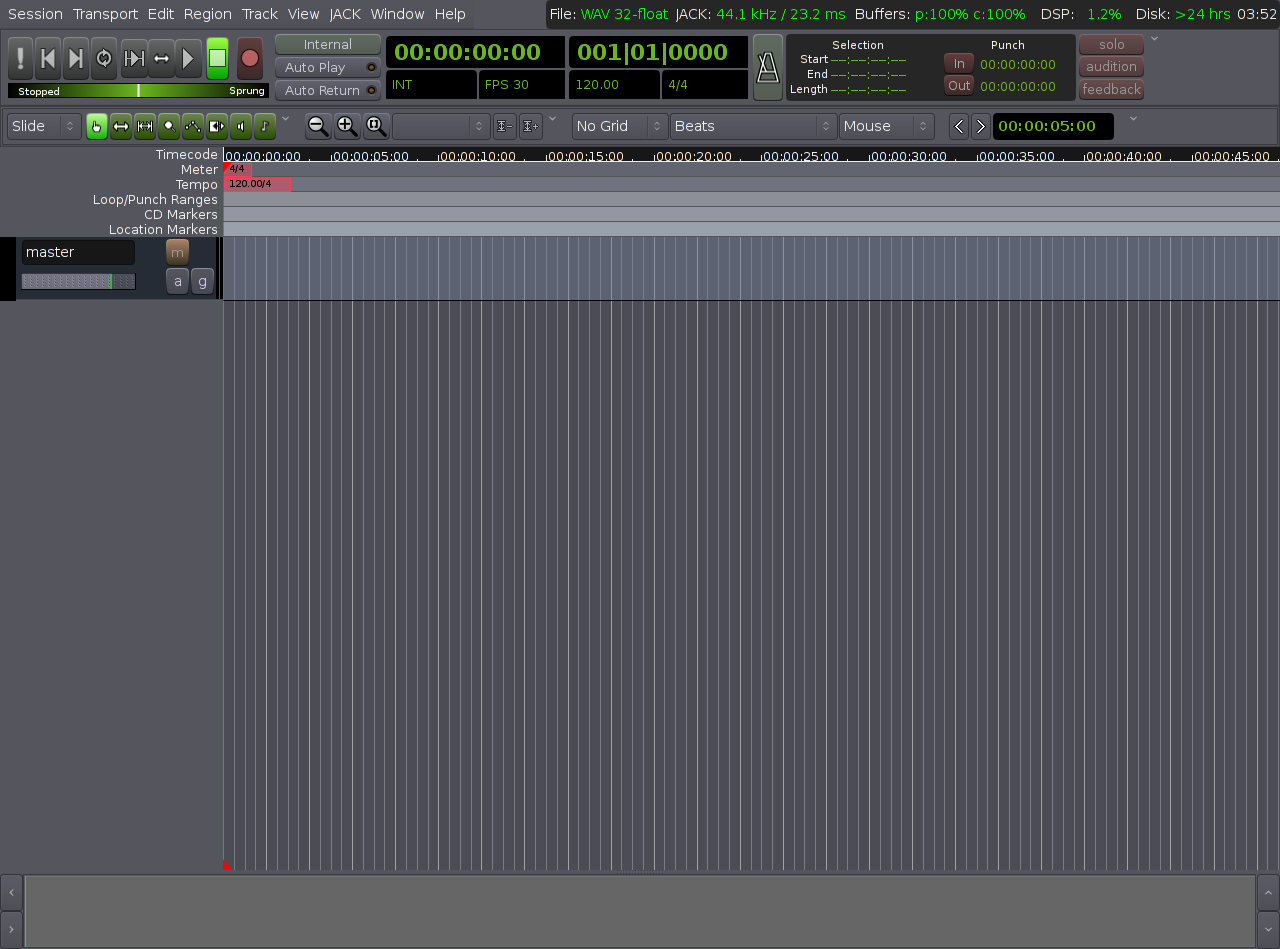
\includegraphics[scale=0.3]{screenshots/editor.png}
\end{center}
\caption{\ldots and finally: the editor!}
\label{fig:editor}
\end{figure}

\section{Adding a track and connecting it up}

The next step is to add a track to our session so that we have
something to record onto.  Choose \menu{Track,Add Track or Bus...}
from the menu at the top of the editor window.  This will bring up a
dialogue box, as shown in Figure~\ref{fig:quickstart-add-track-or-bus}.

\screenshot{add-track-or-bus.png}{`Add Track or Bus' dialogue}{fig:quickstart-add-track-or-bus}

For now, leave the options as they are; this will create a single
monophonic audio track.  This track must now be connected to the sound
card so that it can record incoming audio.

Perhaps the easiest way to connect up this new track is to open its
editor mixer strip.  Do this now by pressing \key{Shift,E} or
choosing \menu{View,Show Editor Mixer} from the main menu.  The top of
the mixer strip that appears looks like that in
Figure~\ref{fig:top-of-mixer-strip}.

\screenshot{top-of-mixer-strip.png}{Top part of a mixer strip}{fig:top-of-mixer-strip}

At the top of this mixer strip there are three main buttons.  The
first, labelled `Audio 1' (the name of the track) can be clicked on to
open a menu of options for the track.  The second, marked `1' is the
input selector, and the third, marked $\phi$, is a button to invert
the track's signal.

In order to look at the connections to the input of this track,
left-click on the button marked `1' to open the input \emph{port
  matrix}, as shown in Figure~\ref{fig:input-port-matrix}.

\screenshot{input-port-matrix.png}{Input port matrix}{fig:input-port-matrix}

The port matrix is the main interface that Ardour offers for
connecting things together.  In our example matrix, the left-hand side
shows a set of ports that generate audio data; these correspond to the
sound card inputs, outputs of Ardour busses and tracks, and other
things that may exist on the system.  Different groups of these ports
can be seen by choosing one of the tabs on the far left-hand side of
the dialogue.

At the bottom of the dialogue is the input to our track.

In the example matrix, there is a green dot at the intersection of the
`L' part of `in $1+2$' and the `Audio 1 in' port.  This means that the
input of the `Audio 1' track hardware input 1.  Change this
connection, if necessary, by clicking on the square which corresponds
to the input to record from.  At this point, the Audio 1 meter should
display any signal that is being sent into the sound card.  If this is
not working, something has gone wrong.

\section{Recording}

At this point, Ardour is receiving a signal from some external sound
source via the sound card.  It is now possible to make a test
recording.  Click the record-enable buttons (red buttons with a pink
circle) in both the `Audio 1' track controls and the main transport
controls (shown in Figures~\ref{fig:track-controls} and
\ref{fig:transport-controls} respectively, then click `Play' to start
the transport.

\screenshot{track-controls.png}{Track controls area}{fig:track-controls}
\screenshot{transport-controls.png}{Main transport controls}{fig:transport-controls}

Ardour is now recording; the play-head will move, and a red rectangle
will be drawn where the recording is taking place.  Make a noise with
your external sound source!  When you have finished recording, click
the Stop button in the transport controls area.  You should now have a
region containing your recording on the `Audio 1' track, as in
Figure~\ref{fig:recorded-one-region}.

% \screenshot{recorded-one-region.png}{Editor window after recording a region}{fig:recorded-one-region}

\section{Playing back your recording}

Now we can play back the audio that you have just recorded.  First,
you will need to move the playhead back to a point before your
recorded region.  Perhaps the easiest way to do this is to click
somewhere within the rulers area of the editor window.

% some picture of where this is, or a back-link to the editor window

Once the playhead is located before your recording, click the `Play'
button (or press the spacebar on the keyboard) to start playback.  You
should hear your recording through your monitor speakers or
headphones.

\section{Adding another track as an overdub}

Now we can experiment further by adding an overdub to the first
recording.  First, add a new track, as we did before, and connect it
up to the input on your soundcard which your source is connected to.

Now, record-enable the new track, move the playhead to before the
previously recorded region, make sure the session is record-enabled
and start the transport (by clicking `Play' or pressing the spacebar).
You should hear the previously-recorded audio on your monitor system
while the new recording is in progress.  Record something suitable
over the top of your first region.

We now have two tracks of recorded data; you might like to add some
more!

\section{Mix-down}

We will now assume that you want to do a mix-down of your magnum opus
into a stereo WAV file.  Such a file could later be converted to an
MP3, or burned to CD, or simply played-back as-is by some other media
player on your computer.  

First, we need to mix the tracks that you have recorded so that they
sound as you want them to.  We will cover much more advanced mixing
and processing later, but for now we will just set the relative levels
of the two tracks.  The easiest way to do this is to open the
\emph{mixer} window, either by selecting \menu{Window,Mixer} or by
pressing \key{Alt,M}.  The mixer window is shown in Figure~\ref{fig:mixer-window}.

% \screenshot{mixer-window.png}{The mixer window}{fig:mixer-window}

Here you will see a mixer strip for each track that you have recorded,
and a `master' strip.  The signals for each track flow from the
recordings on disk, through the appropriate strip, and they are then
mixed together and passed through the master strip.  The bottom half
of each mixer strip contains a \emph{fader}; this controls the level
of each track.  You can adjust the levels of each of your recordings
by dragging the mixer strip; the green marker indicates 0dBFS (`unity
gain'), at which the level of the track will be unaltered from the
recording.

Play back your recordings from the editor window, and experiment with
the levels in the mixer window until you have a sound that you are
happy with.


\section{Export}

The final step is to export our recording into a stereo WAV file.
Ardour's export options are extensive, but for now we will keep it
simple.  Choose \menu{Session,Export,Export to Audio Files} from the
editor menu, and the \emph{Export} dialogue will open, as shown in
Figure~\ref{fig:export-dialogue}.

First, we have to specify the format that we will export in.  Fill in
the \emph{Label} field with some name like `WAV for CD', then click
the \button{New} button beside the Format entry in the dialogue, and
click on \button{CD}, \button{Lossless (linear PCM)}, \button{WAV} and
\button{44.1kHz} entries.  Then click \button{Save} to save the export
preset.  Enter some label for the export in the \emph{Location}
section, then click \button{Export}.  Ardour will mix your session
down to a WAV file and save it in the \directory{export} subdirectory of
your session folder.


\chapter{Tracks and busses}

The basic building blocks of Ardour's signal flow are \emph{tracks}
and \emph{busses}.

Both are built on the same foundation; a bus's functionality is a
subset of a track's.  Both can pass audio and MIDI data, apply
processing and perform various signal routing operations.  The
difference with a track is that can record and play back data.

\section{Track and bus basics}

\subsection{Types}

An Ardour track can be either `audio' or `MIDI'.  The only real
difference between the two is the type of data that the track will
record and play back.  Either type of track can \emph{pass} either
type of data.  Hence, for example, one might have a MIDI track that
contains an instrument plugin; such a track would contain MIDI data,
but would produce audio, since the instrument would turn the one into
the other.

In Ardour~3 busses are only used for audio.

\subsection{Adding and removing tracks}

A track or bus can be added to a session in various ways:

\begin{itemize}
\item Choose \menu{Track,Add Track or Bus\ldots} from the main menu.
\item Right-click in an empty part of the track controls area.
\item Click the $+$ button underneath the list of tracks in the mixer.
\end{itemize}

Any of these actions will open the \emph{Add Track or Bus} dialogue,
as shown in Figure~\ref{fig:add-track-or-bus}.

\screenshot{add-track-or-bus.png}{Add Track or Bus dialogue}{fig:add-track-or-bus}

From here, you can select firstly the number of tracks or busses to
add, and the type; audio track, MIDI track or bus.  There are also
some options, which vary depending on the type of thing you are
creating.

These options are:
\begin{itemize}
\item Configuration (for audio tracks and busses) --- this is the
  number of input and outputs the track is set up with.  You can
  always change these counts later.
\item Track mode (for audio tracks) --- this can be `normal', `non-layered' or `tape'.
\todo{I have no idea what non-layered nor tape modes do}
\item Group --- tracks and busses can be put into groups so that a
  selected range of operations are applied to all members of a group
  at the same time (selecting record enable, or editing, for example).
  This option allows you to specify an existing group to add the new
  track(s) or bus(ses) to, or to create a new group to put the new
  things in.
\item Instrument (for MIDI tracks) --- this is a short-cut to allow you to create a MIDI
  track with an instrument plugin already added to it.  You can
  achieve the same effect by creating a MIDI track with no plugins and
  adding it yourself; this option just makes things slightly quicker.
\end{itemize}

Adding tracks will add them to both the editor and mixer windows; the
editor window shows the timeline, with any recorded data, and the
mixer shows just the processing elements of the track (its plugins,
fader and so on).

Tracks and busses can be removed by selecting them, right-clicking and
choosing `Remove' from the menu.  A warning dialogue will pop up, as
\emph{track removal cannot be undone}; use this option with care!

\chapter{Unfiled miscellany}

\section{MIDI binding maps}

MIDI binding maps provide a way to set up how a physical control
surface (such as a Behringer BCF2000 or Mackie Control) interacts with
Ardour.  An XML file is created to describe the mapping, and Ardour
loads it.  Maps for several devices are supplied with Ardour:

\begin{itemize}
\item Behringer BCF2000 (in native and Mackie Control modes)
\item Behringer DDX3216
\item Korg nano-Kontrol
\item M-Audio Oxygen 8 v2
\item M-Audio Axiom 25
\item Roland SI-24
\item EMU Xboard61
\end{itemize}

This chapter describes the format of the maps and how to create your own.


\subsection{File basics}

MIDI bindings are stored in files with the suffix \texttt{.map}
attached to their name. The minimal content looks like this:

\begin{listing}
<?xml version="1.0" encoding="UTF-8"?>\\
<ArdourMIDIBindings version="1.0.0" name="The name of this set of bindings">\\
</ArdourMIDIBindings>\\
\end{listing}

The remainder of the file gives the bindings themselves, describing
the two parts of each binding: MIDI data that your controller sends,
and things that Ardour does in response.

A binding is an XML node called \texttt{<Binding>}.  The properties of the
node give the details of the binding.  

%The Basic Concept

%Since the beginning of time (well, sometime early in the 2.X series), Ardour has had the concept of identifying each track and bus with a remote control ID. This ID uniquely identifies a track or bus so that when messages arrive from elsewhere (MIDI or OSC), we can determine which track or bus they are intended to control. Ardour has a number of ways of assigning remote control IDs, but they don't really matter very much when creating MIDI binding maps, so we won't discuss that here. You just need to know that there is a "first track" and its remote control ID is 1, and so on.

\subsection{Finding out what your MIDI control surface sends}

This is the most complex part of the job, but it's still not very hard.
You need to connect the control surface to an application that will
show you the information that the device sends each time you modify a
knob, slider, button etc.  There are a variety of such applications;
most notably gmidimon and kmidimon.  You can also use Ardour for this:

\begin{enumerate}
\item Select \menu{Window,MIDI Tracer}.
\item Choose `MIDI Control In' from the Port selector.
\item Use the MIDI connection matrix to connect Ardour's
MIDI Control In port to the MIDI port that your control surface is
sending data in on.
\item Then watch the control surface's MIDI data appear
in the MIDI Tracer window as you twiddle knobs or push buttons.
\end{enumerate}


\subsection{Describing MIDI in the binding file}

The properties for specifying the MIDI data in a \texttt{<Binding>}
node are as follows:

\begin{itemize}
\item \texttt{channel="c" ctl="m"} --- a continuous controller message $m$ arriving on channel $c$.
\item \texttt{channel="c" note="n"} --- a note-on message for note $n$ arriving on channel $c$.
\item \texttt{channel="c" pgm="p"} --- a program change message to program $p$ arriving on channel $c$.
\item \texttt{channel="c" pb="0"} --- a pitch bend message on channel $c$.
\item \texttt{sysex="a b c ..."} --- a sequence of MIDI bytes $a$, $b$, $c$ and so on that make up a system-exclusive message (as hexadecimal bytes)
\item \texttt{msg="a b c ..."} --- an arbitrary sequence of MIDI bytes $a$, $b$, $c$ and so on (as hexadecimal bytes)
\end{itemize}

\subsection{Binding to Ardour}

There are two basic kinds of bindings you can make between a MIDI
message and something inside Ardour. The first is a binding to a
specific parameter of a track or bus. The second is a binding to a
function that will change Ardour's state in some way. 


\subsubsection{Binding to track/bus controls}

A track/bus binding is a binding to an individual track or bus inside
Ardour.  Such a binding requires the name of the property to control,
which can be one of:

\begin{itemize}
\item \texttt{/route/gain}
\item \texttt{/route/solo}
\item \texttt{/route/mute}
\item \texttt{/route/recenable}
\item \texttt{/route/send/gain}
\item \texttt{/route/plugin/parameter}
\end{itemize}

It then requires an address.  For track-level controls (solo, gain, mute, record-enable), the address is one of:

\begin{itemize}
\item A number --- the remote control ID of a track or bus
\item The letter \emph{B} followed by a number --- the remote control ID of a track or bus within the current bank
\item One or more words --- the name of a track or bus
\end{itemize}

For send, insert and plugin controls, the address consists of a track
or bus address followed by a number identifying the plugin or send
(starting from 1).  For plugin parameters, there is an additional third
component: a number identifying the plugin parameter number (starting
from 1).

For solo and mute bindings, you can also add \texttt{momentary="yes"} after the
control address. This is useful primarily for note-on bindings --- when
Ardour gets the note-on it will solo or mute the targetted track or
bus, but then when a note-off arrives, it will un-solo or un-mute it.

The specification of a track or bus binding is put inside a \texttt{uri} property.  For example,

\begin{listing}
<Binding channel="1" ctl="20" uri="/route/gain 2">
\end{listing}

binds a control change on controller 20, channel 1 to the gain of track 2.  As another example

\begin{listing}
<Binding channel="4" note="20" uri="/route/recenable B5">
\end{listing}

binds a note-on for note 20 on channel 4 to the record-enable state of
the 5th track in the current bank.



\subsection{Binding to Ardour `functions'}

Rather than binding to a specific track/bus control, it may be useful
to have a MIDI controller able to alter some part of Ardour's state. A
binding definition that does this looks like this:

\begin{listing}
<Binding channel="1" note="13" function="transport-roll"/>
\end{listing}

In this case, a note-on message for note number 13 (on channel 1) will
start the transport rolling. The following function names are
available:

\begin{itemize}
\item \texttt{transport-stop} --- stop the transport 
\item \texttt{transport-roll} --- start the transport `rolling'
\item \texttt{transport-zero} --- move the playhead to the zero position 
\item \texttt{transport-start} --- move the playhead to the start marker 
\item \texttt{transport-end} --- move the playhead to the end marker 
\item \texttt{loop-toggle} --- turn on loop playback 
\item \texttt{rec-enable} --- enable the global record button 
\item \texttt{rec-disable} --- disable the global record button 
\item \texttt{next-bank} --- move track/bus mapping to the next bank (see `banks' below) 
\item \texttt{prev-bank} --- move track/bus mapping to the previous bank (see `banks' below) 
\end{itemize}

\subsection{Binding to Ardour `actions'}

You can also bind a sysex or arbitrary message to any of the items
that occur in Ardour's main menu (and its submenus). The best place to
look for the (long) list of how to address each item is in your
keybindings file, which will contain lines that look like this:

\begin{listing}
(gtk\_accel\_path "<Actions>/Editor/temporal-zoom-in" "equal")
\end{listing}

To create a binding between an arbitrary MIDI message (we'll use a
note-off on channel 1 of MIDI note 60 (hex) with release velocity 40
(hex)), the binding file would contain:

\begin{listing}
<Binding msg="80 60 40" action="Editor/temporal-zoom-in"/>
\end{listing}

The general rule, when taken an item from the keybindings file and
using it in a MIDI binding is to simply strip the <Action> prefix of
the second field in the keybinding definition.

\subsection{Banks and banking}

Because many modern control surfaces offer per-track/bus controls for
far fewer tracks and busses than many users want to control, Ardour
offers the relatively common place concept of `banks'. Banks to allow
you to relatively easily control any number of tracks and/or busses
regardless of how many faders/knobs etc. your control surface has. To
use banking, the control addresses must be specified using the bank
relative format mentioned above (`B1' to identify the first track of a
bank of tracks, rather than `1' to identify the first track).

One very important extra piece of information is required to use
banking: an extra line near the start of the list of bindings that
specifies how many tracks/busses to use per bank. If the device has 8
faders, then 8 would be a sensible value to use for this. The line
looks like this:

\begin{listing}
<DeviceInfo bank-size="8"/>
\end{listing}

In addition, you probably want to ensure that you bind something on
the control surface to the next-bank and prev-bank functions,
otherwise you and other users will have to use the mouse and the GUI
to change banks, which rather defeats the purpose of the bindings.

\subsection{Motorised controls}

If your surface's controls are motorised, so that Ardour can move your physical controls,
add

\begin{listing}
motorised="yes"
\end{listing}

to your \texttt{<DeviceInfo>} node, so that it reads something like

\begin{listing}
<DeviceInfo bank-size="8" motorised="yes">
\end{listing}

This will make Ardour more efficient in handling your controls.

\subsection{A complete (though muddled) example}

\begin{listing}
<?xml version="1.0" encoding="UTF-8"?>\\
<ArdourMIDIBindings version="1.0.0" name="pc1600x transport controls">\\
<DeviceInfo bank-size="16"/>\\
<Binding channel="1" ctl="1"   uri="/route/gain B1"/>\\
<Binding channel="1" ctl="2"   uri="/route/gain B2"/>\\
<Binding channel="1" ctl="3"   uri="/route/send/gain B1 1"/>\\
<Binding channel="1" ctl="4"   uri="/route/plugin/parameter B1 1 1"/>\\
<Binding channel="1" ctl="6"   uri="/bus/gain master"/>\\
\\
<Binding channel="1" note="1"  uri="/route/solo B1"/>\\
<Binding channel="1" note="2"  uri="/route/solo B2" momentary="yes"/>\\
\\
<Binding channel="1" note="15"  uri="/route/mute B1" momentary="yes"/>\\
<Binding channel="1" note="16"  uri="/route/mute B2" momentary="yes"/>\\
\\
<Binding sysex="f0 0 0 e 9 0 5b f7" function="transport-start"/>\\
<Binding sysex="f0 7f 0 6 7 f7" function="rec-disable"/>\\
<Binding sysex="f0 7f 0 6 6 f7" function="rec-enable"/>\\
<Binding sysex="f0 0 0 e 9 0 53 0 0 f7" function="loop-toggle"/>\\
\\
<Binding channel="1" note="13" function="transport-roll"/>\\
<Binding channel="1" note="14" function="transport-stop"/>\\
<Binding channel="1" note="12" function="transport-start"/>\\
<Binding channel="1" note="11" function="transport-zero"/>\\
<Binding channel="1" note="10" function="transport-end"/>\\
</ArdourMIDIBindings>\\
\end{listing}

Please note that channel, controller and note numbers are specified as
decimal numbers in the ranges 1-16, 0-127 and 0-127 respectively.


\section{The processor list}

Each track or bus in Ardour has a list of \emph{processors} that
operate on the audio or MIDI signal passing through it.  The operation
of the processor list is illustrated in
Figure~\ref{fig:basic-processor-list}.

\begin{figure}[ht]
\begin{center}
\includegraphics{diagrams/basic-processor-list.pdf}
\end{center}
\caption{Basic structure of a track or bus}
\label{fig:basic-processor-list}
\end{figure}

Audio or MIDI data arrives from a file on disk, or from the input
ports, depending on the monitoring settings that are in effect.  It is
then passed through each processor in sequence, before being panned
and sent to the output ports.

The term `processor' is a very general one.  It includes:

\begin{itemize}
\item Plugins (LADSPA, LV2, VST etc.)
\item Sends and returns
\item The fader
\item The meter
\end{itemize}

Some processors are shown in the Ardour's mixer strip, and some are
hidden.  Consider the example mixer strip shown in Figure~\ref{fig:processor-box}.

\screenshot{processor-box.png}{The processor box}{fig:processor-box}

Here we see five visible processors; they are:

\begin{enumerate}
\item `Autotalent'; a plugin.  This is coloured red to indicate
  that it is pre-fader.
\item The fader.  This is where the mixer fader's gain is applied.
\item Invada High Pass; a plugin.
\item 4-band parameteric; another plugin.  The symbol between the
  high-pass and the parametric indicates that the signal is being
  split from mono to stereo, as the parametric is a stereo plugin.
\item TAP dynamics; another plugin.
\end{enumerate}

Some processors are not shown on this list:

\begin{itemize}
\item The meter; a processor which assesses the level of the signal at
  its point in the processor chain.
\item A sned to the main output.
\item A send to the monitor bus, if one is being used.
\end{itemize}


\section{Operations on the processor list}

The processor list in each mixer strip can be manipulated in several
different ways.

Firstly, processors can be re-ordered using drag-and-drop.  Dragging a
processor allows it to be moved around within the chain, or copied to
another processor list on another track or bus.

Secondly, processors can be enabled or disabled.  To the left of the
name of each processor is a small LED symbol; if this is lit-up, the
processor is active.  Clicking on it will deactivate the processor.
It will still pass audio or MIDI signals, but they will not be
affected.

Finally, processors can be added to or removed from the chain.
Right-clicking the processor list does three things:

\begin{itemize}
\item A gap is opened up to indicate the location of the click.  The
  gap shows where any new processors will be inserted.
\item The processor under the click is selected.
\item A menu is presented giving options of what to do.
\end{itemize}

From the menu, some new processors can be inserted.  These can be
plugins, sends or internal sends.  The selected processor can also be
deleted or copied.



\section{Monitoring}

The basic role of a track is to record and playback audio or MIDI
data.  In some situations, however, it is useful to be able to get a
track to pass live audio or MIDI from its input to its output.
Consider, for example, a track with a couple of plugins that is being
used for a vocal recording.  It may be desirable to listen to the
processed live vocal from the output of the track, either before or
during recording.  Generally speaking, the passing of live input data
around Ardour is called \emph{monitoring}.


\subsection{Different ways of monitoring}

There are three basic ways in which monitoring may be approached:

\begin{itemize}
\item External monitoring --- this is where Ardour plays no role in
  monitoring at all.  Perhaps the recording set-up has an external
  mixer which can be used to set up monitor mixes, or perhaps the
  sound-card being used has some `listen to the input'-style feature.
  This approach often has the advantage of zero or near-zero latency.
  On the other hand it requires external hardware, and the monitoring
  settings are not saved with the session.

% XXX diagrams here

\item JACK-based `hardware' monitoring --- some sound cards have the
  ability to mix signals from their inputs to their outputs with zero-
  or low-latency.  Furthermore, on some cards these features can be
  controlled by JACK\@.  This is a nice arrangement, if the sound card
  supports it, as it combines the convenience of having the monitoring
  controlled by Ardour with the low latency operation of doing it
  externally.

\item Software monitoring --- this where all monitoring is performed
  by Ardour; it makes track inputs available at track outputs, under
  the influence of various controls.  This approach will almost always
  have more routing flexibility than JACK-based monitoring.  The
  disadvantage is that there will be a latency between the input and
  the output which will depend mainly on the JACK buffer size that is
  being used.

\end{itemize}

\subsection{Setting up monitoring}

There are three main settings which affect how monitoring is
performed.  The first is `Record monitoring handled by' in the
\emph{Audio} tab of the \emph{Ardour Preferences} dialogue.  There are
two or three options here, depending on the capabilities of your
hardware:

\begin{itemize}
\item \emph{ardour} --- Ardour handles monitoring itself (software monitoring).
\item \emph{audio hardware} --- Ardour does no monitoring at all, and
  assumes you will do it yourself (external monitoring)
\item \emph{JACK} --- Ardour will ask JACK to, in turn, ask the sound
  card to handle monitoring.  This option is only available if it is
  supported by your sound card (hardware monitoring).
\end{itemize}

The other two settings are more complex; one is `Tape machine mode',
in the same dialogue, and the other is `Monitoring automatically
follows transport state (`auto-input')' setting in \emph{Session
  Properties}.

Monitoring is also somewhat dependent on the state of the track's
record-enable button, the session record enable button, and whether or
not the transport is rolling.


\subsection{Monitoring in software or hardware monitoring modes}

If Ardour is set to `external monitoring', the explanation of Ardour's
monitoring behaviour is simple: it does not do any.  In the other two
modes, things are more complex.


\subsection{Monitoring in non-tape-machine mode}

This section describes what happens when Ardour is \emph{not} set to
tape-machine mode.

Consider first the case when a track is record-enabled.  In this
situation, it will always monitor the live input \emph{unless} the
session is \emph{not} record-enabled, auto-input is enabled, and the
transport is rolling.  

When a track is not record-enabled, the track will play back its
contents from disc \emph{unless} the transport is stopped and
auto-input is enabled.  In this case, the track monitors its live
input.


\subsection{Monitoring in tape-machine mode}

In tape-machine mode, things are slightly simpler; when a track is
record-enabled, its behaviour is the same as in non-tape-machine mode:
it will always monitor the live input \emph{unless} the session is
\emph{not} record-enabled, auto-input is enabled, and the transport is
rolling.

When a track is not record-enabled, however, the track will always
just play back its contents from disk; the live input will never be
monitored.


\todo{Some more rational explanation of why things are like this}
\todo{Metering!}


\section{Tracks and busses in detail}

\begin{ddanger}
This section goes into somewhat unhealthy detail about how tracks and
busses operate internally.  It may be of interest to almost nobody.
\end{ddanger}

Tracks and busses in Ardour share a common basis; they are both
pathways through which audio and MIDI data can pass, experiencing
various processing and distribution along the way.  The only real
difference between a track and a bus is that a track can either obtain
its input from a JACK port, or from files on disk; a bus has no disk
files, so only processes signals coming from other parts of Ardour, or
from other programs via JACK\@.

Internally, Ardour uses the term `route' to describe a bus, with a
track being a superset of the route's functionality (to include the
parts which read from and write to disk).  This chapter uses the word
`route' to indicate either a track or a bus, where the two have the
same behaviour.

Not all of the processing that signals experience as they travel
through routes is visible in the Ardour user-interface. The visible parts
are the plugins, the fader, the meter and (if present) the panner.
There are other invisible processes that happen to support Ardour's
internal operation.  Figure~\ref{fig:route-in-detail} gives a
representation of the entire pathway of a route.

% XXX: panning
\begin{figure}[ht]
\begin{center}
\includegraphics{diagrams/route-in-detail.pdf}
\end{center}
\caption{Detailed view of a route}
\label{fig:route-in-detail}
\end{figure}

Audio or MIDI data starts from either a set of JACK ports or a disk
file.  Busses always take their initial data from JACK ports, and
tracks can do either depending on monitoring settings.  It is possible
for tracks and busses to have no input, in which case the signal
starts off as silence.

If a track is recording, data is taken straight from the JACK input
ports and recorded; no processing on track will have any effect on the
recorded signal.

The signal then enters the processing chain.  Internally, this chain
is a set of `processors' connected in series.  Some processors are put
in place by Ardour, and some are at the whim of the user.

\subsection{Export}

% XXX

\subsection{Internal return}

This is the point at which internal send signals from other routes
appears in the route being sent to.  This processor gathers signals
from all its connected sends and mixes them with the signal in the
route at that point.

\subsection{Monitor control}

% XXX

\subsection{Monitor send}

The monitor send is an internal send which sends the route's signal,
whever it is located, to the monitor bus.  The monitor send is located
in different places, depending on the settings for AFL and PFL\@.

\subsection{Meter}

The meter processor passes signals unaltered, but meters them on the
way through.  It can be moved around depending on the meter point settings.

\subsection{User processors}

These are the `conventional' user-visible processors: plugins and
internal sends to other tracks or busses.

\subsection{Amp}

This is a gain-control element which is controlled by the fader.

\subsection{Main out}

This processor takes the route's signal, optionally pans it, and then
passes it to a set of JACK ports; this represents the main output of
the route.


\appendix
\chapter{Advanced JACK setup}
\label{ap:advanced-jack}

\section{Using JACK with multiple sound cards}

If you want to set up JACK to use multiple sound cards at the same
time, there are a number of options:

\begin{enumerate}

\item Use the \texttt{alsa\_in} and \texttt{alsa\_out} clients (Linux and ALSA only)

If you are using JACK on Linux and want to use additional devices that
have ALSA driver support (i.e. most PCI, USB and Bluetooth devices),
then this is the best option.

\texttt{alsa\_in} and \texttt{alsa\_out} are two clients written by
Torben Hohn that make a single ALSA device appear as a set
of JACK ports. They both use Erik de Castro Lopo's libsamplerate
library to do any resampling required to keep the audio in sync as the
clocks of each device drift over time.

To use them, you start JACK as normal. Then you start an instance of
\texttt{alsa\_in} or \texttt{alsa\_out} for each additional device
(and `direction') that you want to use. \texttt{alsa\_out} will create
a set of ports representing the playback capabilities of the device,
and \texttt{alsa\_in} will represent the capture/recording
capabilities. These two clients must be run inside a terminal window; 
there is no GUI for either of them. They both take arguments very much
like those of the JACK ALSA backend, with some additional controls
that affect the way that resampling is done. Full details are
available in the manual pages for each client, which you can read in a
terminal window with the command

\begin{listing}
man alsa\_in
\end{listing}

This page covers both clients, since their arguments are identical.

Note that you can use these clients even if you are running JACK with
a FFADO-supported device. The requirement for ALSA support only
applies to the extra devices you want to use, not the one that JACK
itself is using.

\item Use the JACK2 audio adapter(s) (Jack2 only)

% XXX More information is needed on this option

\item Using OS facilities to merge devices into a single pseudo-device

Both OS~X and Linux provide ways to configure your machine so that it
appears to have a new audio device that is actually a combination of
one or more real devices. You can use this approach to create the
configuration you want to use and then start up JACK using that new
`pseudo' device.

\begin{itemize}
\item OS X

You must perform these steps as a user with administrative
privileges. The first thing to do is to open up
\menu{Applications,Utilities,Audio/MIDI Setup}. Go to the main menu
bar, click on \button{Audio} and then select \emph{Open aggregate device
editor}. Follow the simple instructions to add the each desired
playback or capture device to your new aggregate device. Then pick a
name for the new device. This is the name you will also use to choose
the device for use with JACK\@.

Note that there are quite a few subtle bugs with Apple's `aggregate
device' facilities. Various things can happen that will cause the
device to lose all of its playback channels or all of its capture
channels, for example. If this happens, it is generally necessary to
close all applications that are using any audio devices, and quite
often a reboot is required.

Starting with JACK2 version 1.9.6, the CoreAudio backend can now
dynamically create `aggregate devices' when needed (like when the -C
and -P arguments are used to specify the separated input and output
devices).

\item Linux

You will need to use a text editor to create or add to your
\texttt{~/.asoundrc} file. This file is read by any ALSA application
(including JACK, if its using the ALSA backend) and can be used to
define pseudo-devices of many different kinds. The key idea here is
that you're going to define a new pseudo-device composed of 2 or more
other devices. In our example, we'll just focus on 2 devices being
merged into 1, where both devices have just 2 channels in and
out. This is the text you need to make sure is in \texttt{~/.asoundrc} (below,
we describe what this does):

\begin{listing}
pcm.merge \{\\
    type multi;\\
    slaves.a.pcm hw:0\\
    slaves.a.channels 2;\\
    slaves.b.pcm hw:1\\
    slaves.b.channels 2;\\
    bindings.0.slave a;\\
    bindings.0.channel 0;\\
    bindings.1.slave b;\\
    bindings.1.channel 0;\\
    bindings.2.slave a;\\
    bindings.2.channel 1;\\
    bindings.3.slave b;\\
    bindings.3.channel 1;\\
\}\\
\end{listing}

Lets see what this does:

\begin{itemize}

\item It defines a new audio pseudo-device called `merge'. You can use
  this name anywhere you might use the name of an ALSA audio device,
  such as \texttt{hw:0} or \texttt{hw:HDA} or \texttt{hw:DSP} or
  \texttt{plughw:1}.
\item It names \texttt{hw:0} as the first component (or `slave') of
  this pseudo-device (\texttt{slave.a.pcm}) and \texttt{hw:1} as the
  second component (\texttt{slave.b.pcm})
\item It states that the pseudo-device will use 2 channels from the
  first component and 2 channels from the 2nd component.
\item The lines containing \texttt{binding.} list, in order, which
  channel of which component will correspond to the 4 channels of the
  pseudo-device. In the mapping shown above, the first channel comes
  from the first component, then the 2nd channel from the 2nd
  component, the 3rd from the first component and the 4th from the
  second component.

\end{itemize}

Note that numbering of devices and channels in ALSA starts at zero,
not one.

The most important and complex part of the above definition is the
channel mappings defined by the bindings lines. A full channel mapping
definition consists of a pair of a lines of the following general
form:

\begin{listing}
bindings.CHANNEL\_OF\_PSEUDO\_DEVICE.slave SLAVE\_DEVICE\_THAT\_WILL\_PROVIDE\_THIS\_CHANNEL\\
bindings.CHANNEL\_OF\_PSEUDO\_DEVICE.channel CHANNEL\_OF\_SLAVE\_DEVICE\_THAT\_WILL\_PROVIDE\_THIS\_CHANNEL
\end{listing}

So the specific pair of lines:

\begin{listing}
bindings.0.slave a;\\
bindings.0.channel 0;
\end{listing}

mean that `channel 0 of the pseudo-device will correspond to channel 0
of the first slave device'. Obviously by playing with this definition
you can create all sorts of wierd and wonderful mappings from the real
physical device channels to the pseudo-device channels. You probably
don't want to do that, though. The example above shows the most common
example: take the first $N$ channels from the first device, and the
second $M$ channels from the second device.

In theory, the above is enough to define a new pseudo-device, but many
applications, including JACK's ALSA backend, also want to open a
"control device" associated with the audio playback device. This is
where they can find out (and possibly control) various hardware
parameters associated with the device. Unfortunately there is no way
to merge these together in the same way, so we have to provide a
"dummy" control device definition that will keep such applications
happy. This definition looks like this:

\begin{listing}
ctl.merge \{\\
    type hw\\
    card 0\\
\}
\end{listing}

Notice that name following the \texttt{ctl.} text must be the same as
the name following \texttt{pcm.} in the device definition above. The
control device definition we've given here effectively means `if you
want to open the control device associated with ``merge'', open the
control device associated with the first installed audio/MIDI
device'. This probably isn't right of course --- `merge' involves two
cards --- but it will generally work just fine.

You can use this same approach to merge more than 2 devices - the
resulting \texttt{pcm.DEVICE-NAME} specification will obviously
include more lines. You can also use different devices than we did
above, where we just used the first and second installed card.

Note that you are likely to be better off using \texttt{hw:CARD} device names,
rather than \texttt{hw:N} names, when defining a `multi' pseudo-device, as
explained here. But further note that if you are using multiple
instances of the same type of audio hardware (say, 4 RME Multiface
devices), you will have to use \texttt{hw:N} because every card will have the
same \texttt{CARD} name. In fact, with such hardware, it may be very
difficult to ensure that \texttt{hw:0} always refers to the same audio
interface, because there is no ALSA name that uniquely defines a
particular PCI slot. This is currently an unsolved problem when using
multiple identical devices. If you use PCI (or PCIe or PCIx or other
derivatives of PCI) devices, the chances are that the first card will
always be the same one, and so forth, so its not likely to be an
issue. If you use several identical USB devices, it may be a more
significant problem.

\item Using the \texttt{-P} and \texttt{-C} arguments to a JACK backend

Several JACK backends, including the ALSA, FFADO and CoreAudio
versions, support the \texttt{-P} and \texttt{-C} arguments that can
be used to specify two different devices, one for playback and one for
capture/recording. You cannot use this to merge multiple devices for
playback or capture. This approach will not do any clock drift
correction, so as the two devices drift over time, you may get
glitches in the audio stream. Nevertheless, it can be an easy if
unreliable way to set up JACK so that, for example, it records from a
USB microphone and plays back via a builtin audio device.

When using \texttt{-P} or \texttt{-C} to specify different devices, do
not use the \texttt{-d} argument (which specifies a single device) and
do not use the \texttt{-D} argument (which tells JACK to configure a
device for playback and capture).

\end{itemize}
\end{enumerate}



\end{document}



